\subsubsection{Testbench và Kết quả mô phỏng Address Mux}

\textbf{a. Mô tả Testbench} \\
\begin{itemize}
    \item \textbf{Kiểm tra tính phản hồi tức thời}: Xác nhận ngõ ra \texttt{addr\_out} cập nhật ngay khi tín hiệu chọn \texttt{sel} 
    thay đổi mà không phụ thuộc vào xung clk.
    \item \textbf{Mô phỏng chu kỳ máy}: 
        \begin{itemize}
            \item Thiết lập \texttt{sel = 1} để kiểm tra luồng địa chỉ từ Program Counter (giai đoạn Fetch).
            \item Thiết lập \texttt{sel = 0} để kiểm tra luồng địa chỉ từ Instruction Register (giai đoạn Execute).
        \end{itemize}
    \item \textbf{Kiểm tra tính độc lập}: Thay đổi dữ liệu tại ngõ vào không được chọn 
    để đảm bảo ngõ ra vẫn giữ nguyên giá trị từ nguồn đã chọn.
\end{itemize}

\textbf{b. Mã nguồn Testbench}
\begin{lstlisting}[language=Verilog, caption={Ma nguon Testbench kiem tra Address Mux}]
`timescale 1ns / 1ps

module tb_address_mux();

    // Khai bao tham so do rong bit
    parameter W = 32;

    reg  [W-1:0] pc_addr;
    reg  [W-1:0] ir_addr;
    reg          sel;
    wire [W-1:0] addr_out;

    // Khoi tao module Address Mux voi tham so W 
    address_mux #(.WIDTH(W)) uut (
        .pc_addr(pc_addr),
        .ir_addr(ir_addr),
        .sel(sel),
        .addr_out(addr_out)
    );

    initial begin
        $display("-----------");
        $display(" Time|sel|pc_addr|ir_addr|addr_out");
        $display("-----------");
        $monitor("%10t|%b|%h|%h|%h", 
                 $time, sel, pc_addr, ir_addr, addr_out);

        // Khoi tao gia tri ban dau
        pc_addr = 32'h0000_1000; // Dia chi lenh 
        ir_addr = 32'h0000_ABCD; // Dia chi toan hang 
        sel = 0;

        //Test chon ir_addr 
        #10; sel = 0; 
        //Test chon pc_addr 
        #10; sel = 1;

        //Thay doi pc_addr khi dang chon pc_addr
        #10; pc_addr = 32'h0000_1004;

        //Thay doi ir_addr khi dang chon pc_addr (addr_out khong doi)
        #10; ir_addr = 32'h0000_EEEE;

        //Chuyen sang chon ir_addr
        #10; sel = 0;

        #10;
        $display("-----------");
        $display("Hoan thanh mo phong Address Mux!");
        $finish;
    end
endmodule
\end{lstlisting}

\textbf{c. Sơ đồ mạch RTL} \\
Sơ đồ RTL xác nhận khối được tổng hợp thành một bộ dồn kênh 2-sang-1 đơn giản, với đường dẫn dữ liệu từ hai nguồn đầu vào hội tụ tại một bộ chọn được điều khiển bởi tín hiệu \texttt{sel}.

\begin{figure}[H]
    \centering
    % Thay 'mux_rtl.png' bang ten file anh cua ban
    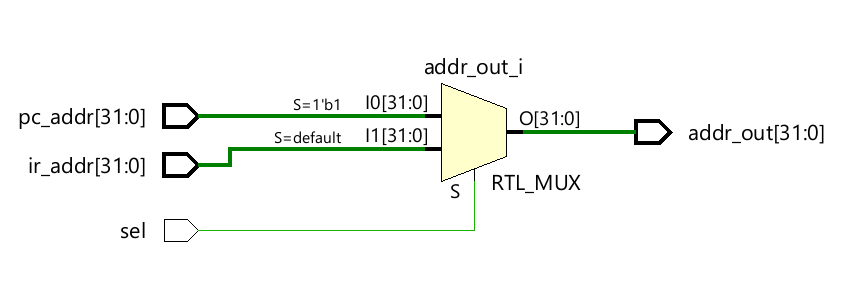
\includegraphics[width=0.6\textwidth]{sodoadd.png} 
    \caption{Sơ đồ mạch RTL của khối Address Mux}
    \label{fig:mux_rtl}
\end{figure}

\textbf{d. Kết quả xuất ra màn hình} \\
Kết quả Console minh chứng cho logic chuyển mạch tức thời của module.

\begin{figure}[H]
    \centering
    % Thay 'mux_console.png' bang ten file anh console cua ban
    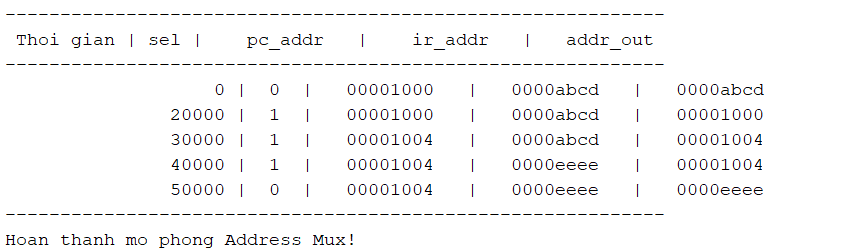
\includegraphics[width=0.8\textwidth]{consoleadd.png} 
    \caption{Kết quả chạy Testbench Address Mux trên Console}
    \label{fig:mux_console}
\end{figure}

Dựa trên bảng kết quả, tại thời điểm \texttt{sel = 1}, \texttt{addr\_out} luôn bám sát giá trị của \texttt{pc\_addr}. 
Khi thay đổi \texttt{ir\_addr} trong khi \texttt{sel} vẫn bằng 1, ngõ ra hoàn toàn không bị ảnh hưởng.

\textbf{e. Giản đồ sóng} \\

\begin{figure}[H]
    \centering
    % Thay 'mux_waveform.png' bang ten file anh waveform cua ban
    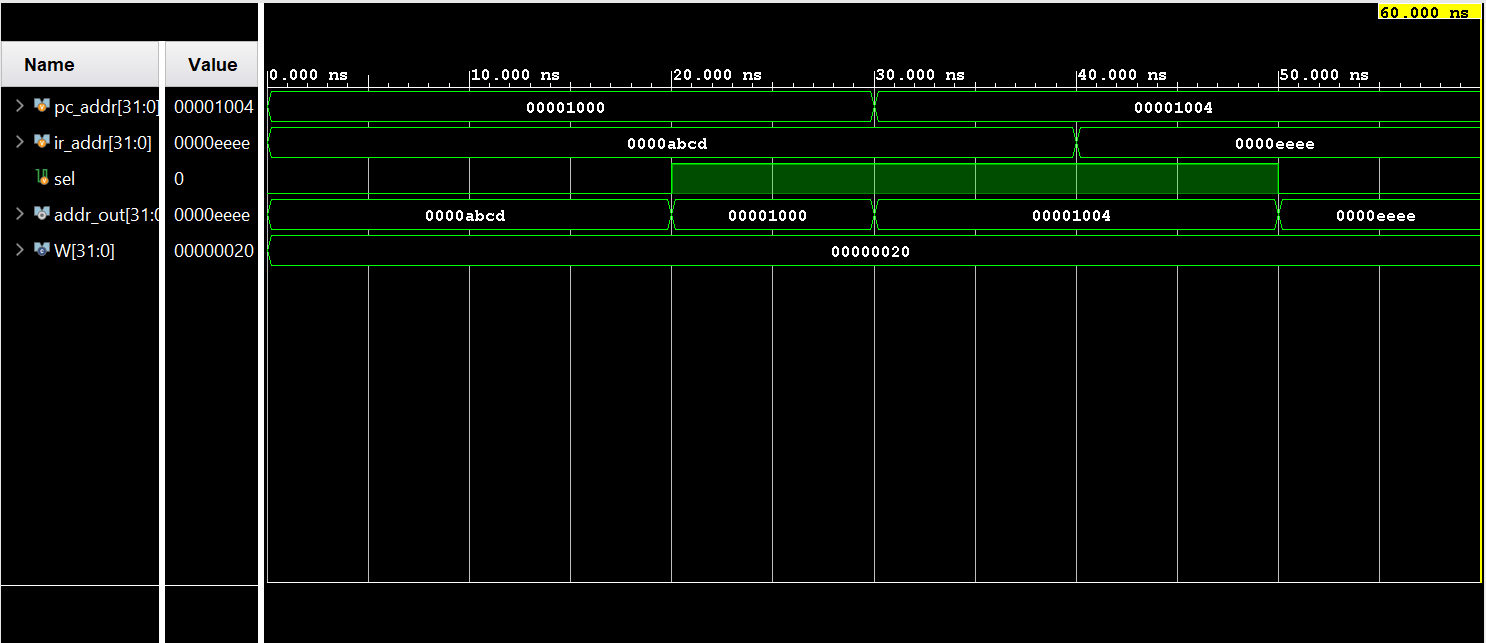
\includegraphics[width=\textwidth]{waveadd.png} 
    \caption{Giản đồ sóng mô phỏng khối Address Mux}
    \label{fig:mux_waveform}
\end{figure}
